\documentclass{beamer}
\usepackage{natbib}
\usepackage{hyperref}
\usepackage[utf8]{inputenc}
\usetheme{Madrid}
\usepackage{amsthm}
\usepackage{amsmath}
\usepackage{amsfonts}
\usepackage{subcaption}


\newcommand{\len}{\text{len}}
\newcommand{\aslv}{\arg\text{solve}}
\newcommand{\diag}[1]{\text{diag}\{#1\}}
\newcommand{\trace}[1]{\text{tr}\left\{#1\right\}}
\newcommand{\expect}[1]{\mathbb{E}[#1]}
\newcommand{\expectb}[1]{\mathbb{E}\left[#1\right]}
\newcommand{\expectw}[2]{\mathbb{E}_{#2}\left[#1\right]}
\newcommand{\prob}[1]{\mathbb{P}(#1)}
\newcommand{\probb}[1]{\mathbb{P}\left(#1\right)}
\newcommand{\var}[1]{\text{Var}(#1)}
\newcommand{\varb}[1]{\text{Var}\left(#1\right)}
\newcommand{\se}[1]{\text{se}(#1)}
\newcommand{\reals}{\mathbb{R}}
% interval
\newcommand{\ii}[1]{A_{#1}}     
% \newcommand{\abs}[1]{\left\lvert#1\right\rvert}
\newcommand{\func}[2]{#1{(#2)}}
\newcommand{\abs}[1]{\lvert#1\rvert}
\newcommand{\absb}[1]{\left\lvert#1\right\rvert}
\newcommand{\rank}[1]{\text{rank}(#1)}
\newcommand{\norm}[1]{\lVert#1\rVert}
\newcommand{\normb}[1]{\left\lVert#1\right\rVert}
\newcommand{\LNorm}[1]{{\lVert#1\rVert}}
\newcommand{\LTwonorm}[1]{{\lVert#1\rVert}_2}
\newcommand{\LTwonormb}[1]{{\left\lVert#1\right\rVert}_2}
\newcommand{\lone}{\ell_1}
\newcommand{\ltwo}{\ell_2}
\newcommand{\innerprod}[2]{\left\langle#1,#2\right\rangle}
\renewcommand{\dim}[1]{\text{dim}{\left(#1\right)}}
\newcommand{\doubleline}[2]{\begin{tabular}{@{}l@{}} #1 \\ #2\end{tabular}}
\newcommand{\tripleline}[3]{\begin{tabular}{@{}l@{}} #1 \\ #2\\ #3\end{tabular}}
\newcommand{\quadline}[4]{\begin{tabular}{@{}l@{}} #1 \\ #2\\ #3\\ #4\end{tabular}}
\newcommand{\abbrv}[2]{#1 (#2)}
\newcommand{\pckg}[1]{\texttt{#1}}

% Notation
\newcommand{\trst}{R}
\newcommand{\trcard}{r}
\newcommand{\trcoef}{{\beta^*}}
\newcommand{\Lassoest}{\hat{\beta}(\lambda)}
\newcommand{\Lassoestarg}[1]{\hat{\beta}(#1)}
\newcommand{\modelset}{\mathcal{M}}
\newcommand{\inprob}{\overset{p}{\to}}
\newcommand{\indist}{\overset{d}{\to}}
\newcommand{\exsgd}{\theta^{\text{sgd}}}
\newcommand{\imsgd}{\theta^{\text{im}}}
\newcommand{\amin}{\text{argmin}}
\newcommand{\amax}{\text{argmax}}


%Information to be included in the title page:
\title[``Plus/minus'' CIs]{``Plus/minus'' confidence intervals and thresholding}
\author[]{P. Zietkiewicz}
\date{\today}



\begin{document}

\frame{\titlepage}

\begin{frame}
	\frametitle{Table of contents}
	\tableofcontents
\end{frame}

\begin{frame}
  \frametitle{Contents}
  \begin{enumerate}
  \item Thresholding
  \item Combining thresholding with plus minus
  \end{enumerate}
\end{frame}

\begin{frame}
  \frametitle{Thresholding}
  \begin{itemize}
  \item $p$ covariates, then $2^p$ models. Define $I = \{1,,2,\dots,p\}$, $J = \{j \in I: \beta_j \ne 0\}$ and $K = \{j \in I: \beta_j = 0\}$. We define a model selection procedure as the estimator $\hat{J} \subseteq I$, which is the set of selected variables. 
  \item $\hat{J}$ is said to have the oracle property if (1) $\prob{\hat{J} = J} \to 1$ and (2) the limiting distribution of its subvector corresponding to the non-zero coefficients is the same as if this subvector was known prior to estimation.
  \end{itemize}
\end{frame}

\begin{frame}
  \frametitle{Asymptotic normality}
  \begin{figure}[h!]
    \centering
    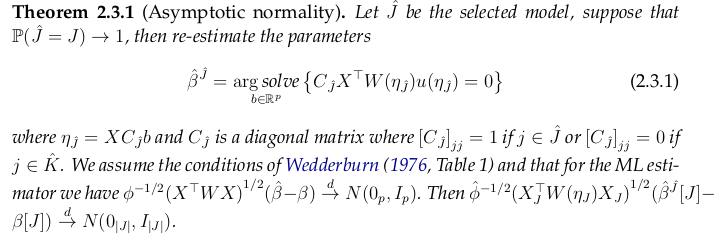
\includegraphics[scale=0.4]{asymp_norm.png}
  \end{figure}
\end{frame}

\begin{frame}
  \frametitle{Wald statistics}
  \begin{itemize}
  \item $\hat{s}_j = O_p(n^{-1/2})$ and $\hat{\beta}_j - \beta_j = O_p(n^{-1/2})$
  \item Define Wald statistic $z_j = \hat{\beta}_j / \hat{s}_j$
  \end{itemize}
  \begin{figure}[h!]
    \centering
    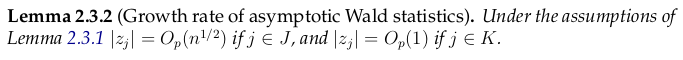
\includegraphics[scale=0.4]{growth.png}
  \end{figure}
\end{frame}

\begin{frame}
  \frametitle{Thresholding for GLMs with ML}
  \begin{figure}[h!]
    \centering
    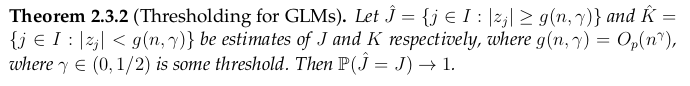
\includegraphics[scale=0.4]{ML_thresh.png}\\
    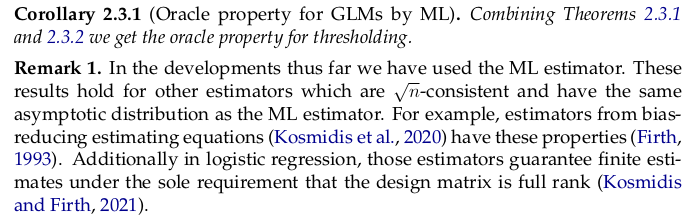
\includegraphics[scale=0.4]{coro_remark.png}
  \end{figure}
\end{frame}

\begin{frame}
  \frametitle{Optimised threshold}
  \begin{itemize}
  \item Wide range of thresholds that would result in a consistent model selection procedures, for example $g(n,1/4) = n^{1/4}$ and $g(n,1/3) = n^{1/3}$ would both suffice.
  \item Let $\gamma_j$ and $g_j$ denote the coefficient-specific rate and threshold function respectively. We propose to minimise the quantity
    \begin{align}
      \omega_j \prob{\abs{z_j} > g_j : j \in K} + (1 - \omega_j) \prob{\abs{z_j} \leq g_j : j \in J} \label{eq:var_select_error}
    \end{align}
    with respect to $\gamma \in (0,1/2)$.
  \item Propose statistic from~\citet{derryberry:2018}
    \begin{align}
      \text{dbic}_j = n\log\left(\frac{z_j^2}{n-p} + 1\right) - \log(n) \label{eq:dbic}
    \end{align}
    and use $\omega_j = I(\text{dbic}_j < 0)$ and $\omega_j = \Phi(-\text{dbic}_j)$ as hard and soft weights respectively.
  \end{itemize}
\end{frame}

\begin{frame}
  \frametitle{Binomial sparse}
  \begin{figure}[h!]
    \centering
    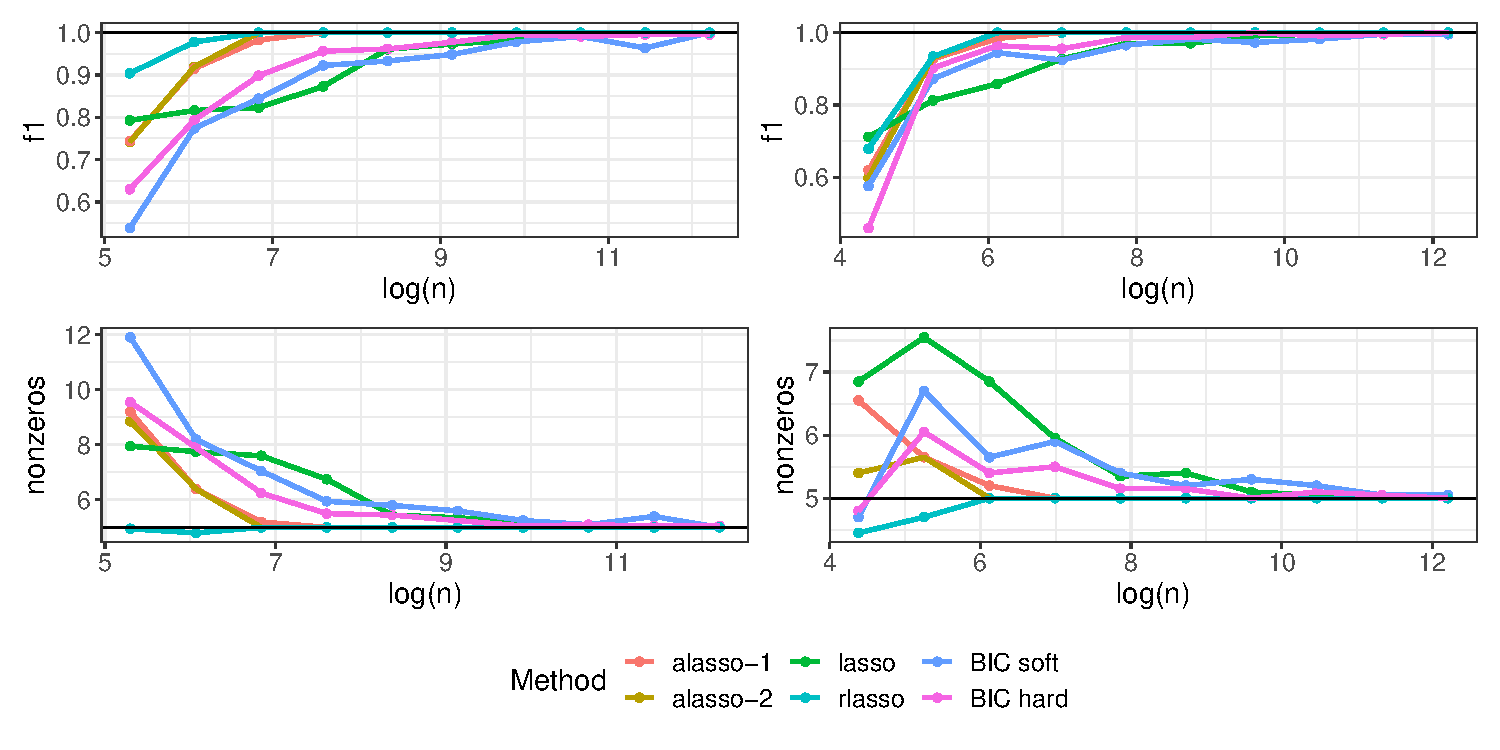
\includegraphics[scale=0.4]{binomial_sparse.pdf}
    \caption{{\footnotesize f1 score and number of non-zero variables in binomial logistic regression with increasing observations with $p=100$ variables and $s=5$ non-zero variables (left) $p=40$ variables and $s=5$ non-zero variables (right).}}
  \end{figure}


\end{frame}

\begin{frame}
  \frametitle{Binomial dense}
  \begin{figure}[h!]
    \centering
    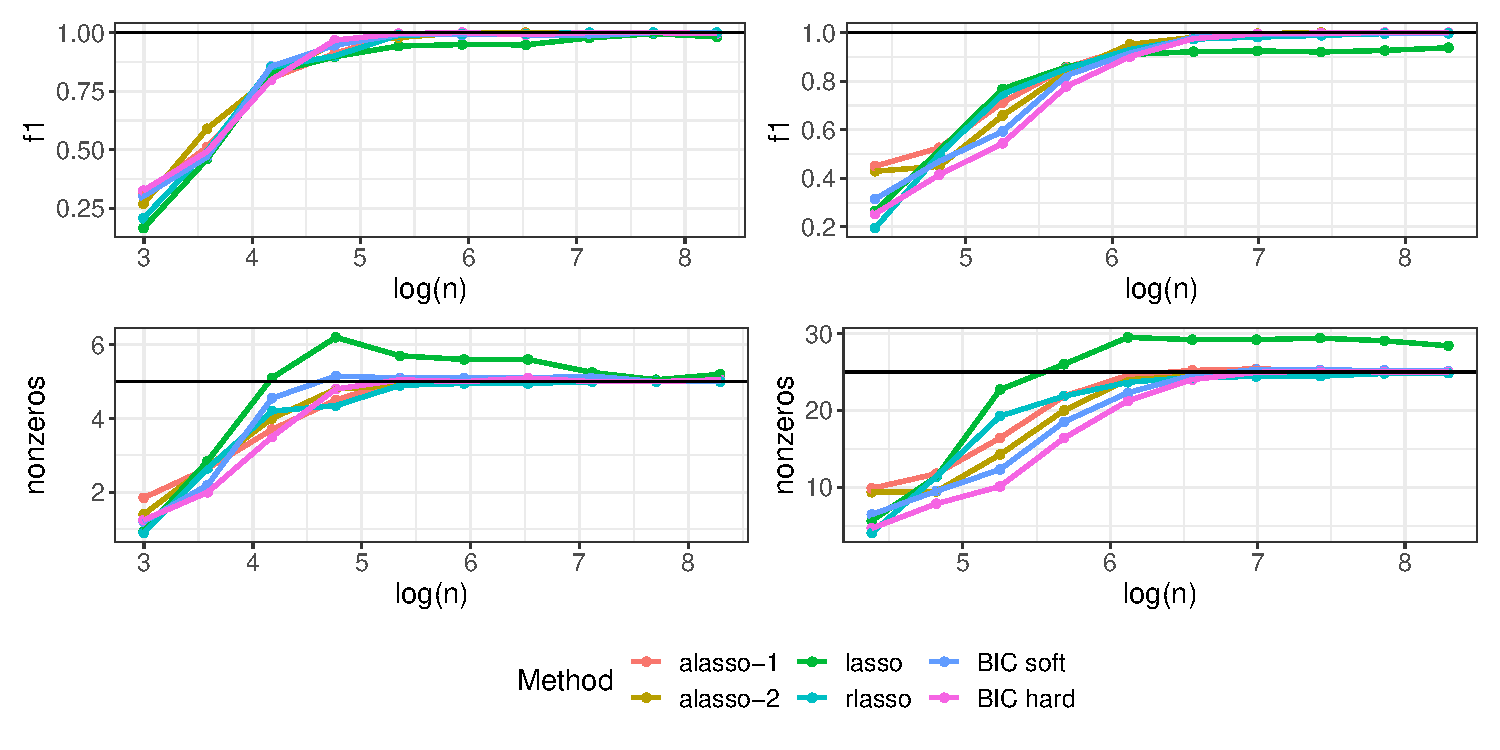
\includegraphics[scale=0.4]{binomial_dense.pdf}
      \caption{{\footnotesize f1 score and number of non-zero variables in binomial logistic regression with increasing observations with $p=10$ variables and $s=5$ non-zero variables (left) $p=40$ variables and $s=25$ non-zero variables (right).}}
  \end{figure}
\end{frame}

\begin{frame}
  \frametitle{Overall conclusion from this}
  Overall, we observe that both soft and hard thresholding procedures converge to the true model, although they may not do so as rapidly as the relaxed or adaptive Lasso in the sparse setting. The performance gap between thresholding and relaxed or adaptive Lasso narrows in denser settings when there is a higher proportion of non-zero entries. The broader point is that thresholding is a viable method for consistent model selection whilst being directly implementable as part of the standard maximum likelihood output, making it more accessible and convenient for practitioners.
\end{frame}

\begin{frame}
  \frametitle{Confidence sets}
  \begin{itemize}
  \item Thresholding allows for the direct use of nonparametric bootstrap for the construction of confidence sets of models, in order to quantify the uncertainty associated with the selected model.
  \item   Confidence sets using the diabetes data~\citep{smith:1988} after 1000 bootstrap iterations for relaxed Lasso (top left) and adaptive Lasso with penalty 2 (top right), soft BIC (bottom left) and hard BIC (bottom right) thresholding. A model is seen as a column of tiles where grey and white indicate whether a variable is included or excluded respectively. Models are shown in descending order of the proportion they appeared in the bootstrap samples.  The dotted red line is at 0.95.
  \end{itemize}
\end{frame}

\begin{frame}
  \frametitle{Confidence sets}
  \begin{figure}[t]
  \centering
  \captionsetup{width=.9\linewidth}
  
  \begin{subfigure}{.5\textwidth}
    \centering
    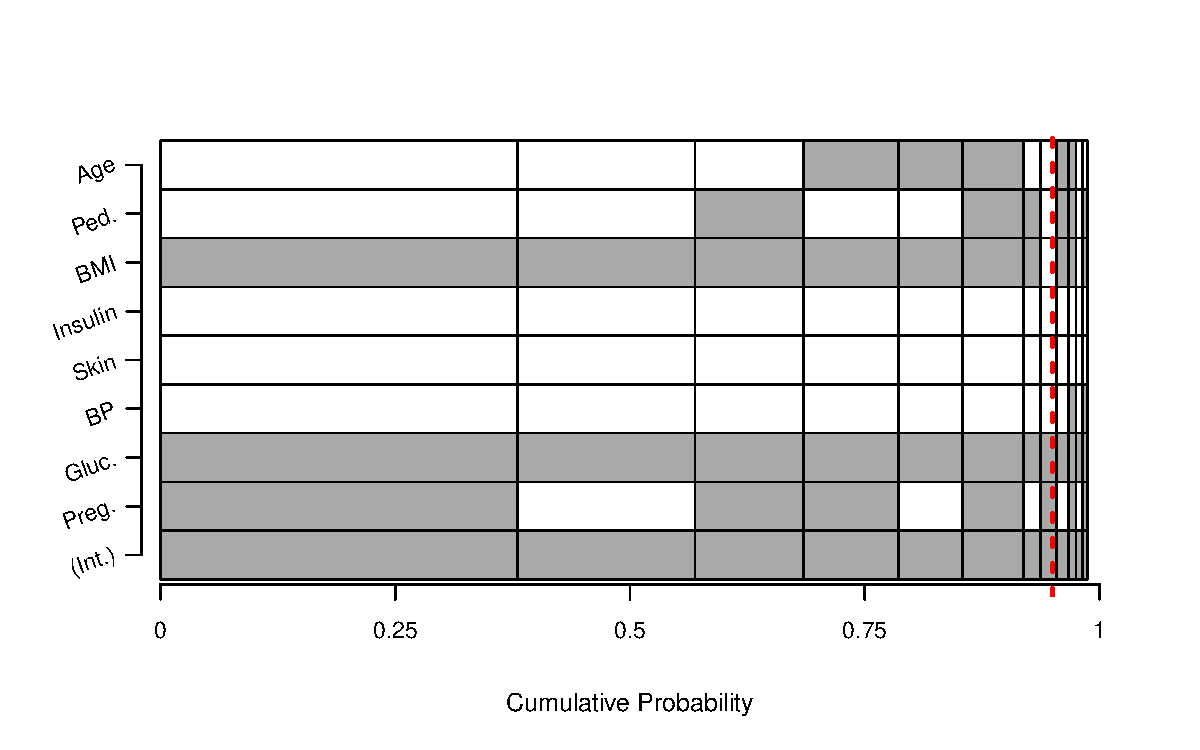
\includegraphics[scale=0.25]{conf_set_elector=ms_lasso.pdf}
    \caption{{\footnotesize Relaxed Lasso.}}
    \label{fig:ms_relaxed}
  \end{subfigure}%
  \begin{subfigure}{.5\textwidth}
    \centering
    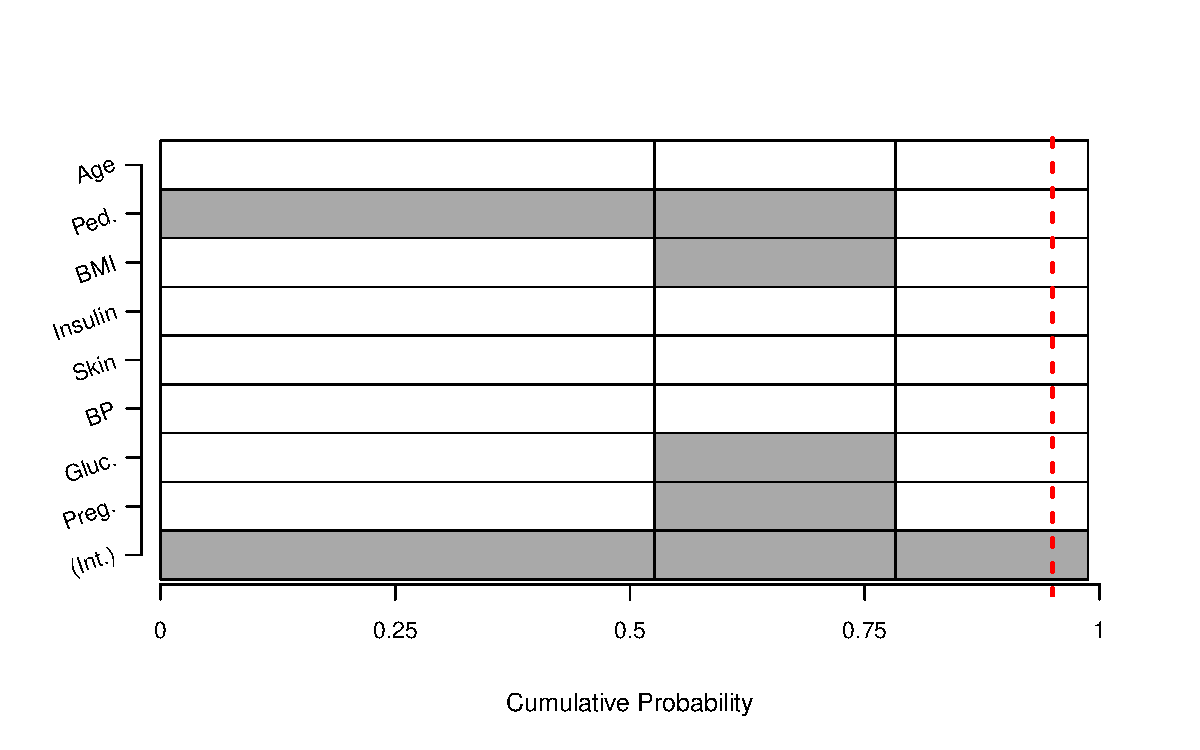
\includegraphics[scale=0.25]{conf_set_elector=ms_adaptive_pen_exp=2.pdf}
    \caption{{\footnotesize Adaptive Lasso with penalty 2.}}
    \label{fig:ms_adaptive_pen_exp=2}
  \end{subfigure}
  
  \begin{subfigure}{.5\textwidth}
    \centering
    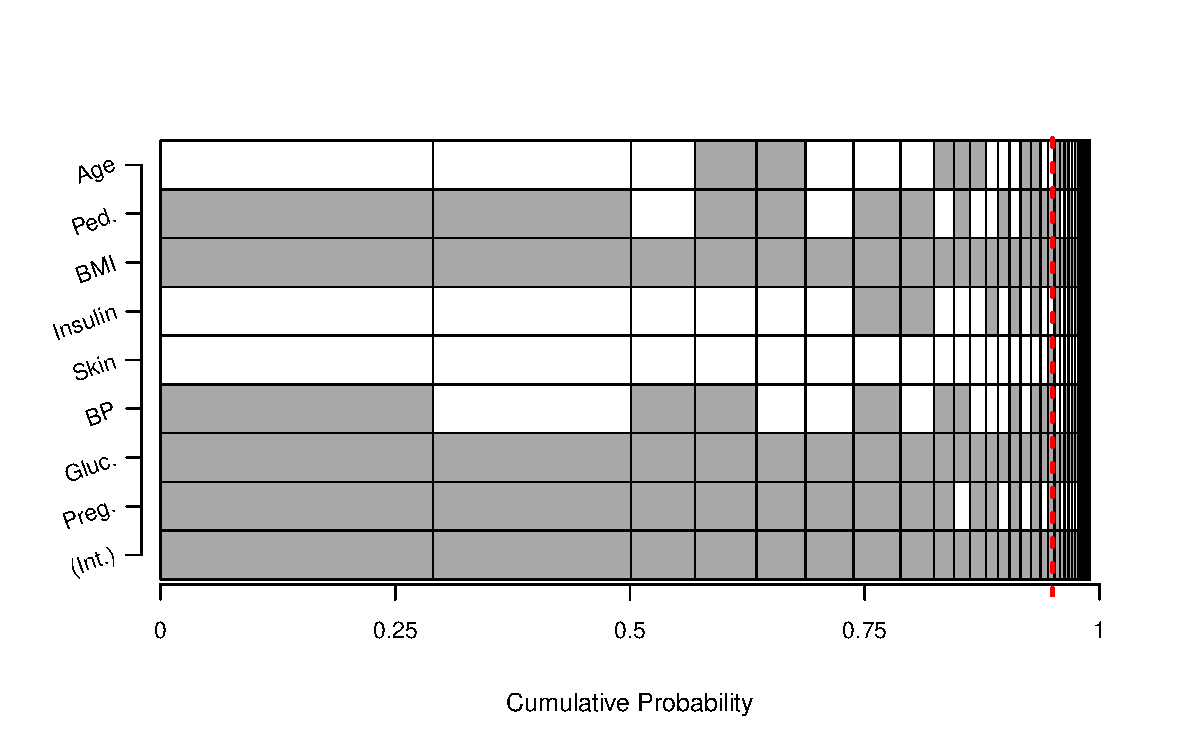
\includegraphics[scale=0.25]{conf_set_elector=ms_thres_w_type=bic_g_type=enhanced2_fixed=FALSE.pdf}
    \caption{{\footnotesize Soft BIC thresholding.}}
    \label{fig:ms_thres_w_type=bic_g_type=enhanced2_fixed=FALSE}
  \end{subfigure}%
  \begin{subfigure}{.5\textwidth}
    \centering
    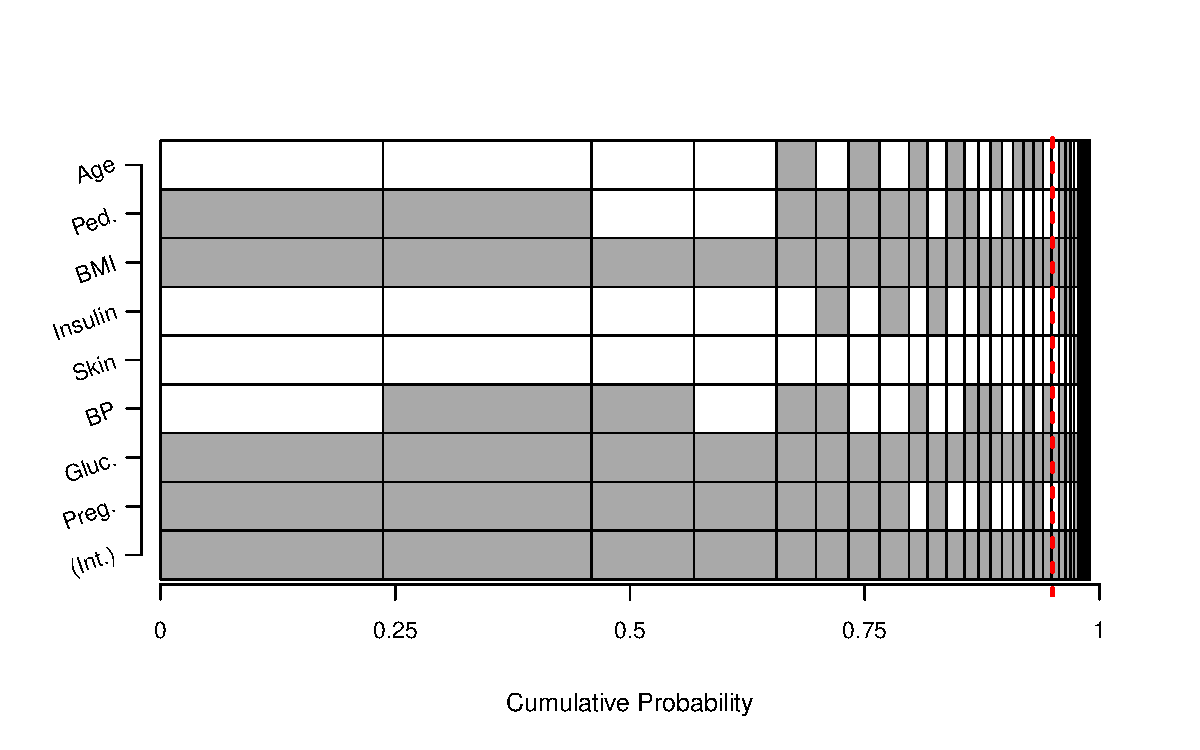
\includegraphics[scale=0.25]{conf_set_elector=ms_thres_w_type=bic_g_type=enhanced2_fixed=TRUE.pdf}
    \caption{{\footnotesize Hard BIC thresholding.}}
    \label{fig:ms_thres_w_type=bic_g_type=enhanced2_fixed=TRUE}
  \end{subfigure}
  \label{fig:combined}
\end{figure}
\end{frame}

\begin{frame}
  \frametitle{Oracle property}
  Distribution of standardized non-zero coefficients after model selection using hard and soft BIC thresholding, Hard BIC and Soft BIC respectively, adaptive Lasso with penalties of 2, 1 and 0.5, Adaptive-2, Adaptive-1 and Adaptive-0.5 respectively. Standard normal distribution is superimposed in black. Data is from binomial logistic regression with $\beta_j = 1$ for $j=1,\dots,5$ and $\beta_j=0$ for $j=6,\dots,40$ with $n=100$ observations and the simulation is repeated for 1000 iterations.
\end{frame}

\begin{frame}
  \frametitle{Oracle property}
  \begin{figure}[t!]
  \centering
  \captionsetup{width=.9\linewidth}
  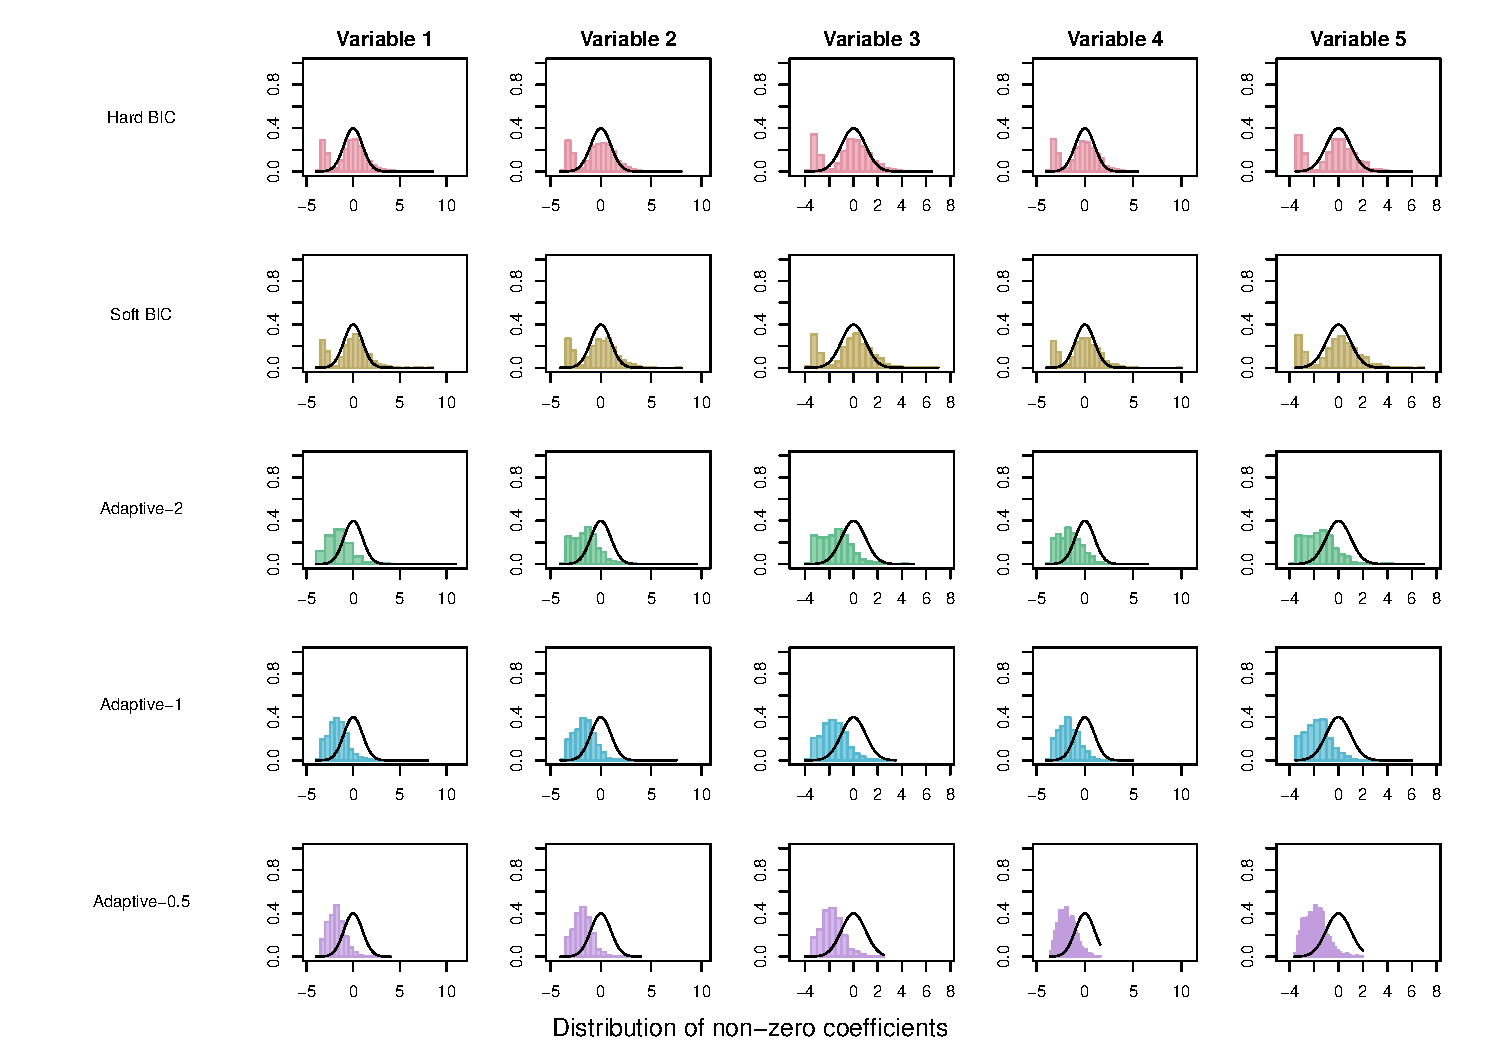
\includegraphics[scale=0.4]{oracle_n100_family-binomial_p40_s5_rho0.pdf}
\end{figure}
\end{frame}



% Old stuff below
\begin{frame}
  \frametitle{Summary of~\citet{chee:2023}}
  \begin{itemize}
  \item Given a dataset \((x_i, y_i)\) for $i\in\{1,\dots,n\}$ where \(x_i \in \mathbb{R}^p\) and \(y_i\) is a realization of the random variable \(Y_i\), and a model parameterized by \(\theta \in \Theta \subseteq \mathbb{R}^p\), with corresponding log-likelihood function $\ell(\theta)$ and we wish to estimate the parameter $\theta$ where the true parameter is $\theta_\star = \amax_{\theta\in\Theta} \expect{\ell(\theta; Y, X)}$. The Fisher information matrix as $F_\star = \expect{-\nabla^2 \ell(\theta_\star; Y, X)}$. The basic iteration of SGD is expressed as
    \begin{align}
      \exsgd_{k+1} = \exsgd_k + \varphi_k \nabla \ell(\exsgd_k; y_k, x_k)\nonumber
    \end{align}
    where \(\varphi_k = \varphi_1 k^{-\varphi}\) is a diminishing learning rate with $\varphi_1 > 0$ and $\varphi\in(0.5, 1]$.
  \item Let $\exsgd_n$ be the one-pass estimator of $\theta_*$.
  \item Advantages of one-pass over multi-pass: (1) Asymptotic covariance matrix is known in closed form (2) Covariance matrix can be bounded by a factor that depends only on the learning rate $\varphi_1$.
  \end{itemize}
\end{frame}


\begin{frame}
  \frametitle{Summary of~\citet{chee:2023}}
  \begin{itemize}
  \item ~\citet{chee:2023} provide methodology to compute very simple confidence intervals using the one-pass estimate of the form
  \begin{align}
    \exsgd_{n,j} \pm 2\sqrt{\frac{\varphi_1^*}{n}} \quad j=1,\dots,p \label{eq:chee_CI}
  \end{align}
  where $\exsgd_{n,j}$ is the $j$th element of $\exsgd_n$ and $\varphi_1^*$ is a tuned hyperparameter. Importantly~\citet[][Theorems 3.1, 3.2]{chee:2023} show that the the confidence intervals~\eqref{eq:chee_CI} are asymptotically valid.
\item Define $\Sigma_* = \varphi_1^2 {(2 \varphi_1 F_* - I)}^{-1} F_*$ where $\varphi_1$ is large enough such that $2\varphi_1 F_* - I \succ 0$. And has eigenvalues
  \begin{align*}
    \text{eigen}(\Sigma_*) = \{\frac{2\varphi_1^2 \lambda_j}{2\varphi_1\lambda_j - 1} : j=1,\dots,p\}
  \end{align*}
  where $\lambda_j$ is the $j$th eigenvalue of $F_*$.
  \end{itemize}
\end{frame}

\begin{frame}
  \frametitle{Summary of~\citet{chee:2023}}
  Results:
  \begin{figure}[h!]
    \centering
    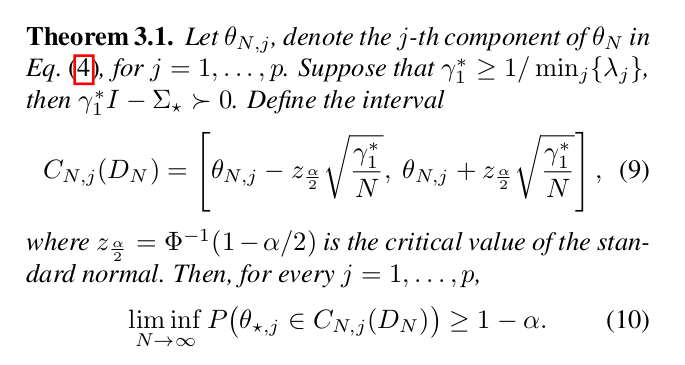
\includegraphics[scale=0.25]{31.png}
    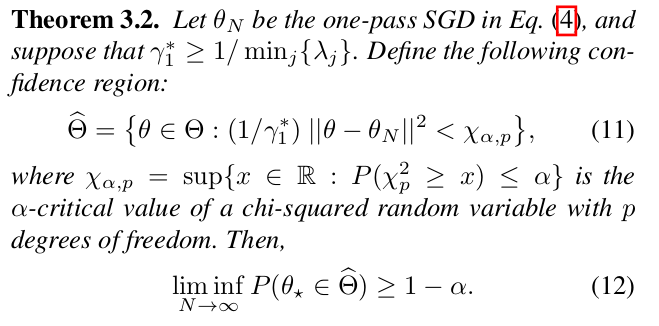
\includegraphics[scale=0.25]{32.png}
  \end{figure}
\end{frame}

\begin{frame}
  \frametitle{Summary of~\citet{chee:2023}}
  Selecting $\gamma_1^*$:
  \begin{figure}[h!]
    \centering
    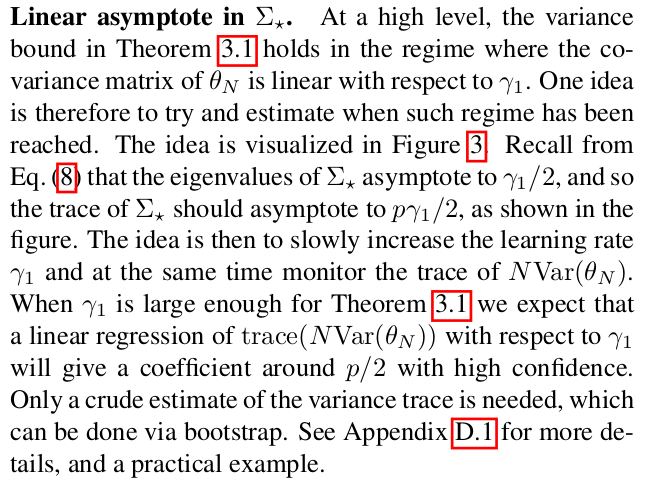
\includegraphics[scale=0.25]{s1.png}
    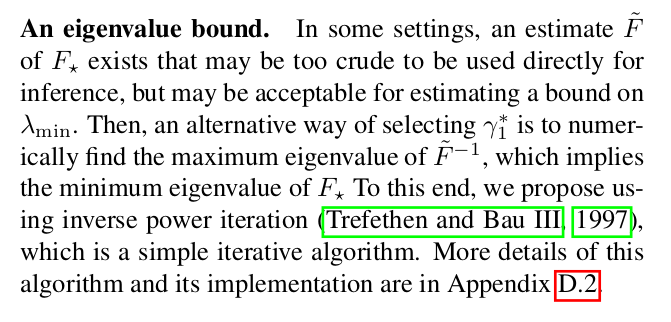
\includegraphics[scale=0.25]{s2.png}
  \end{figure}
\end{frame}


\begin{frame}
  \frametitle{Thresholding and SGD}
  \begin{itemize}
  \item In the context of thresholding we define the Wald statistic
    \begin{align}
      z_{n,j} = \frac{\beta_{n,j}}{\sqrt{\varphi_1^* / n}}. \label{eq:pivot_sgd}
    \end{align}
  \item all the ingredients of our previous Wald statistic. In the numerator if $\beta_j \in J$ we have that $\beta_{n,j}\inprob \beta_j \ne 0$, and if $j \in K$ $\beta_{n,j}\inprob 0$. Then in the denominator we see that $\sqrt{\varphi_1^* / n} = O(n^{-1/2})$. And so,
\begin{align*}
  z_{n,j} = 
  \begin{cases}
    O_p(n^{1/2}) \text{ if } j\in J\\
    O_p(1) \text{ if } j\in K
  \end{cases}
\end{align*}
  \end{itemize}
\end{frame}

\begin{frame}
  \frametitle{Thresholding and SGD}
  \begin{figure}[h!]
    \centering
    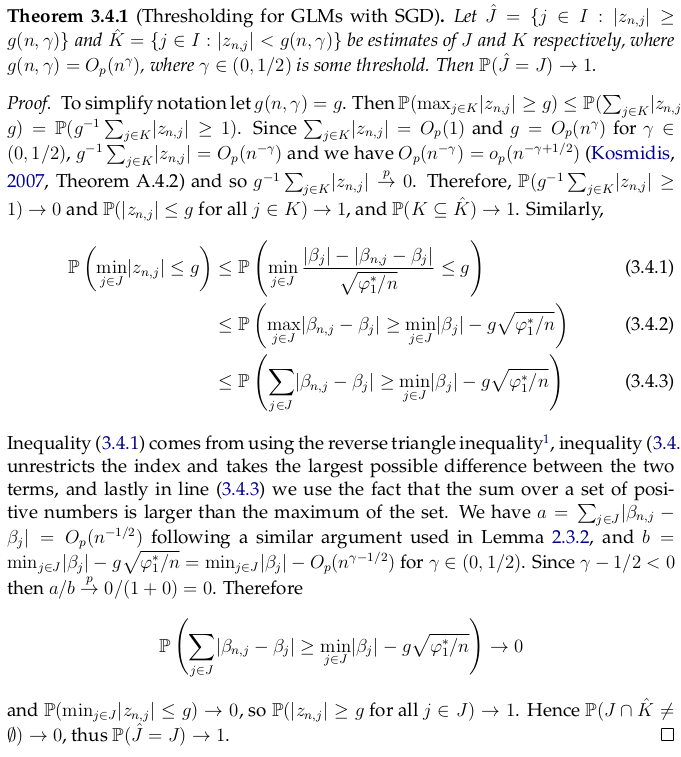
\includegraphics[scale=0.275]{cons_sgd.png}
  \end{figure}
\end{frame}

\begin{frame}
  \frametitle{Simulations}
  \begin{itemize}
  \item First we see how it is possible to generate a confidence sets on the fly. At each step of SGD we estimate the model set using thresholding.
  \item Then look at the oracle property of these estimates.
  \end{itemize}
\end{frame}

\begin{frame}
  \frametitle{Binomial, $p=10$, $s=5$, $n=200$}
    \begin{table}[h]
    \footnotesize
    \centering
    \begin{tabular}{l|r|r}
      Value & Proportion & Cumulative \\
      \hline
       (1,2,3,4,5) &    0.3481 & 0.3481\\
     (1,2,4)  &   0.2873 &  0.6354\\
          ()  &   0.1823 & 0.8177\\
   (1,2,3,4) & 0.1436 & 0.9613\\
       (1,4) & 0.0221 & 0.9834\\
       (2,4) & 0.0110 & 0.9944\\
         (2) & 0.0055 & 0.9999
    \end{tabular}
    \caption{{\footnotesize $n=200$, 95\% CS: \{(1,2,3,4,5), (1,2,4), (), (1,2,3,4)\}}}
  \end{table}
\end{frame}

\begin{frame}
  \frametitle{Binomial, $p=10$, $s=5$, $n=2000$}
  \begin{table}[h]
    \footnotesize
    \centering
    \begin{tabular}{l|r|r}
      Value & Proportion & Cumulative \\
      \hline
      (1,2,3,4,5) & 0.9132 & 0.9132 \\
      (1,3,4,5) & 0.0424 & 0.9556 \\
      () & 0.0162 & 0.9718 \\
      (1,4,5) & 0.0136 & 0.9854 \\
      (4,5) & 0.0050 & 0.9904 \\
      (1) & 0.0030 & 0.9934 \\
      (3) & 0.0030 & 0.9964 \\
      (1,3,5) & 0.0010 & 0.9974 \\
      (3,9) & 0.0010 & 0.9984 \\
      (1,3) & 0.0005 & 0.9989 \\
      (1,9) & 0.0005 & 0.9994 \\
      (9) & 0.0005 & 0.9999 \\
    \end{tabular}
    \caption{{\footnotesize $n=2000$, 95\% CS: \{(1,2,3,4,5), (1,3,4,5)\}}}
  \end{table}
\end{frame}

\begin{frame}
  \frametitle{Binomial, $p=100$, $s=5$, $n=2000$}
  \begin{table}[h]
    \footnotesize
    \centering
    \begin{tabular}{l|r|r}
      Value & Proportion & Cumulative \\
      \hline
      (1,2,3,4,5) & 0.5786 & 0.5786 \\
      (1,2,3,4,5,29) & 0.1571 & 0.7357 \\
      () & 0.1016 & 0.8373 \\
      (1,2,3,4,5,28) & 0.0861 & 0.9234 \\
      (1,2,3,4,5,29,61) & 0.0311 & 0.9545 \\
      (1,3,4,5) & 0.0205 & 0.9750 \\
      (1,4) & 0.0061 & 0.9811 \\
      (1,2,3,4,5,61) & 0.0039 & 0.9850 \\
      (5) & 0.0039 & 0.9889 \\
      (1,2,3,4,5,7) & 0.0028 & 0.9917 \\
      (1) & 0.0028 & 0.9945 \\
      (4) & 0.0022 & 0.9967 \\
      (1,3,4) & 0.0017 & 0.9984 \\
      (1,3) & 0.0011 & 0.9995 \\
      (1,3,5) & 0.0006 & 1.0001 \\
    \end{tabular}
    \caption{{\footnotesize $n=2000$, 95\% CS: \{(1,2,3,4,5), (1,2,3,4,5,29), (), (1,2,3,4,5,28), (1,2,3,4,5,29,61)\}}}
  \end{table}
\end{frame}


\begin{frame}
  \frametitle{Binomial, $p=40$, $s=25$, $n=2000$}
  \begin{table}[h]
    \tiny
    \centering
    \begin{tabular}{l|r|r}
      Value & Proportion & Cumulative \\
      \hline
       (1,2,3,4,5,6,7,8,9,10,11,12,13,14,15,16,17,18,19,20,21,22,23,24,25) & 0.2988 & 0.2988\\
                                                                  ()  & 0.1603& 0.4591\\
    (1,2,3,4,5,6,7,8,9,10,11,12,13,14,15,16,17,18,20,21,22,23,24,25)  &   0.1046 & 0.5637\\
                                                         (2,4,14,22)   &  0.0229 & 0.5866\\
                                                    (2,4,5,13,14,22)    & 0.0193 & 0.6059\\
                                                              (3,14)&     0.0187 & 0.6246\\
              (1,2,4,5,7,8,9,10,11,12,13,14,15,16,20,21,22,23,24,25) &    0.0167 & 0.6413\\
                                                            (3,4,14)  &   0.0146 & 0.6559\\
    (1,2,3,4,5,6,7,8,9,10,11,12,13,14,15,16,17,18,19,20,21,23,24,25)   &  0.0141 & 0.67\\
      (1,2,4,5,6,7,8,9,10,11,12,13,14,15,16,20,21,22,23,24,25)    & 0.0125 & 0.6825\\
      \vdots & \vdots & \vdots \\
    \end{tabular}
    \caption{{\tiny $n=2000$, 95\% CS: \{
        {(1,2,3,4,5,6,7,8,9,10,11,12,13,14,15,16,17,18,19,20,21,22,23,24,25), (), (1,2,3,4,5,6,7,8,9,10,11,12,13,14,15,16,17,18,20,21,22,23,24,25), (2,4,14,22), (2,4,5,13,14,22), (3,14), (1,2,4,5,7,8,9,10,11,12,13,14,15,16,20,21,22,23,24,25), (3,4,14), (1,2,3,4,5,6,7,8,9,10,11,12,13,14,15,16,17,18,19,20,21,23,24,25), (1,2,4,5,6,7,8,9,10,11,12,13,14,15,16,20,21,22,23,24,25), (1,2,4,6,7,8,9,10,11,12,13,14,15,16,17,19,20,21,22,23,24,25), (2,3,4,5,7,9,11,12,13,14,18,22,24,25), (1,2,3,4,5,6,7,8,10,11,12,13,14,15,17,18,20,21,22,23,24,25), (1,2,3,4,5,6,7,8,9,10,11,12,13,14,15,16,17,20,21,22,23,24,25), (1,2,3,4,5,7,8,9,10,11,12,13,14,15,16,17,18,20,21,22,23,24,25), (2,3,14), (3), (1,2,4,7,10,11,12,13,14,15,16,19,20,21,22,23,24,25), (2,14), (3,12,14), (2,4,14,19,22), (1,2,3,4,5,6,7,8,10,11,12,13,14,15,16,17,18,20,21,22,23,24,25), (1,2,3,4,5,6,7,8,9,10,11,12,13,14,15,16,17,18,19,20,21,22,24,25), (2,4,14,20,22), (3,9,12,14), (1,2,3,4,5,6,7,8,9,10,11,12,13,14,15,16,17,18,21,22,23,24,25), (1,2,4,5,7,10,11,12,13,14,15,16,19,20,21,22,23,24,25), (1,2,3,4,5,7,8,9,10,11,12,13,14,15,16,20,21,22,23,24,25), (1,2,4,7,10,11,12,13,14,15,16,19,20,21,22,24,25), (2,4,5,7,9,11,12,13,14,15,18,22,24,25), (1,2,4,5,7,10,11,12,14,15,16,19,20,21,22,23,24,25), (1,2,4,5,7,8,9,10,11,12,13,14,15,16,17,20,21,22,23,24,25), (1,2,4,5,7,9,10,11,12,13,14,15,16,18,19,20,21,22,23,24,25), (2,3,4,5,7,9,11,12,13,14,16,18,22,24,25), (1,2,3,4,7,8,9,10,11,12,13,14,15,16,17,18,20,21,22,24,25), (1,2,4,6,7,9,10,11,12,13,14,15,16,17,19,20,21,22,23,24,25), (1,2,5,7,9,10,11,12,13,14,15,16,18,19,20,21,22,23,24,25), (1,2,3,4,5,7,9,10,11,12,13,14,15,16,18,20,22,24,25), (1,2,4,5,13,14,22), (2,3,4,5,7,9,11,12,13,14,16,18,21,22,24,25), (1,2,3,4,5,6,7,8,10,11,12,13,14,15,16,17,20,21,22,23,24,25), (1,2,3,4,5,6,7,8,9,10,11,12,13,14,15,17,20,21,22,23,24,25), (1,2,3,4,5,7,8,9,10,11,12,13,14,15,16,17,18,20,21,22,24,25), (1,2,5,7,9,10,11,12,13,14,15,16,18,20,21,22,23,24,25), (2,3,4,5,7,9,10,11,12,13,14,15,16,18,21,22,24,25), (2,3,7,9,14,16,18,22,24,25), (1,2,4,7,8,9,10,11,12,13,14,15,16,17,19,20,21,22,23,24,25), (2,3,4,7,9,11,12,13,14,18,21,22,24,25), (2,3,5,7,8,9,14,15,16,18,21,22,24,25), (2,3,5,7,8,9,14,15,16,18,22,24,25), (1,2,3,4,5,6,7,8,9,10,11,12,13,14,15,16,17,18,20,21,22,24,25), (1,2,3,4,7,8,9,10,11,12,13,14,15,16,17,18,20,21,22,23,24,25), (1,2,4,5,7,9,10,11,12,13,14,15,16,18,19,20,22,23,24,25), (2,3,4,7,9,11,12,13,14,18,22,24,25), (1,2,3,7,8,9,14,15,16,18,22,24,25), (1,2,4,5,13,14,18,22,25), (1,2,4,5,7,10,11,12,13,14,15,16,19,20,21,22,24,25), (1,2,4,5,8,9,13,14,16,18,20,22,25), (1,2,4,7,8,10,11,12,13,14,15,16,19,20,21,22,24,25)}
        \}}}
  \end{table}
\end{frame}

\begin{frame}
  \frametitle{Oracle property: $\text{nsim}=300$, Binomial, $n=200$, $p=10$, $s=5$, $B=1$}
  \begin{figure}[h!]
    \centering
    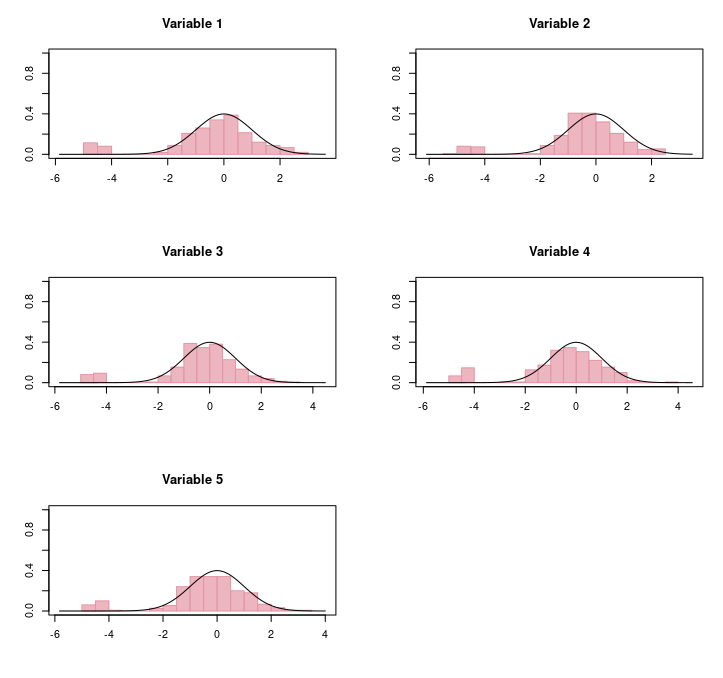
\includegraphics[scale=0.3]{oracle_sgd1.png}
  \end{figure}
\end{frame}

\begin{frame}
  \frametitle{Questions}
  \begin{itemize}
  \item Is there a more efficient way to re-estimate? Using ML is desirable but is that necessary? 
  \item Do you even have to re-estimate? Or could you rerun the SGD algorithm?
  \end{itemize}
\end{frame}

\begin{frame}
  \frametitle{References}
  \bibliographystyle{chicago}
  \bibliography{sgd}
\end{frame}
\end{document}